% !TEX program = xelatex
\documentclass{beamer}

\usepackage{amsmath,booktabs,tabularx,array}
\usetheme{sintef}

% Chinese typography ---------------------------------------------------
\usepackage{xeCJK}
\setCJKmainfont[BoldFont={Microsoft YaHei Bold}]{Microsoft YaHei}
\setCJKsansfont[BoldFont={Microsoft YaHei Bold}]{Microsoft YaHei}
\setCJKmonofont{Microsoft YaHei}
\usefonttheme[onlymath]{serif}

% Traditional Beamer helpers ------------------------------------------
\definecolor{umgold}{RGB}{223,176,28}
\definecolor{umred}{RGB}{170,30,40}
\newcolumntype{Y}{>{\raggedright\arraybackslash}X}
\newcommand{\hl}[1]{\textcolor{maincolor}{\textbf{#1}}}
\newcommand{\gold}[1]{\textcolor{umgold}{\textbf{#1}}}
\newcommand{\smallmuted}[1]{{\small\textcolor{darkgray}{#1}}}
\newcommand{\tightitems}{\setlength\itemsep{2pt}}
\newcommand{\paperbadge}[1]{\textcolor{maincolor}{\scriptsize\textbf{#1}}}
\newcommand{\figbox}[2]{%
  \begingroup
  \setlength{\fboxsep}{2pt}\setlength{\fboxrule}{0.25pt}%
  \fbox{\includegraphics[width=#2\linewidth,height=1.9cm,keepaspectratio]{#1}}%
  \endgroup
}
\newcommand{\awardfig}[1]{%
  \begingroup
  \setlength{\fboxsep}{2pt}\setlength{\fboxrule}{0.25pt}%
  \fbox{\includegraphics[width=\linewidth,height=1.45cm,keepaspectratio]{#1}}%
  \endgroup
}

% Deck identity --------------------------------------------------------
\titlebackgroundcolor{maincolor}
\title{构建人本可信的 AI 系统}
\subtitle{Building Human-Centered, Trustworthy AI Systems}
\course{Teaching / Research Faculty Interview}
\author{樊光瑞 \quad PhD Candidate, Universiti Malaya}
\date{2026 年 5 月 14 日}
\footlinepayoff{}

\begin{document}

\maketitle

% =====================================================================
\section{背景}

\begin{frame}{报告概览}
\begin{itemize}\tightitems
  \item \textbf{个人背景：}学习与工作经历、教学积累、学生培养
  \item \textbf{研究主线：}HCI 驱动的人本可信 AI 系统
  \item \textbf{代表性工作：}四条方向，每条方向给出论文与图示证据
  \item \textbf{未来计划：}课程建设、科研布局、学生培养三年规划
\end{itemize}
\vspace{6mm}
\begin{block}{核心定位}
我的研究关注 AI 系统进入真实场景后，如何改变人的认知、协作、信任与选择。
\end{block}
\end{frame}

\begin{frame}{学习与工作经历}
\begin{itemize}\tightitems
  \item \textbf{2022--2026 \quad 马来亚大学 Universiti Malaya}\\
        \smallmuted{计算机科学博士，预计 2026 年 6 月毕业 \hfill QS 2026 \#58}
  \item \textbf{2018--2026 \quad 太原科技大学}\\
        \smallmuted{讲师，计算机科学与技术学院，本科教学与学生培养}
  \item \textbf{2014--2018 \quad 上海交通大学}\\
        \smallmuted{软件工程硕士，推免入学 \hfill QS 2026 \#47}
  \item \textbf{2010--2014 \quad 华中科技大学}\\
        \smallmuted{数字媒体技术学士，软件学院 \hfill QS 2026 \#319}
\end{itemize}
\vspace{2mm}
\begin{block}{Background}
软件工程训练、课堂教学经验与 HCI/AI 研究方法共同支撑后续研究主线。
\end{block}
\end{frame}

\begin{frame}{教学经历与学生培养}
\footnotesize
\begin{columns}[T]
\begin{column}{0.48\textwidth}
\begin{block}{本科教学}
\begin{itemize}\tightitems
  \item Java Web 开发
  \item Oracle 数据库
  \item 物联网 RFID 技术
\end{itemize}
\end{block}
\begin{block}{学生培养}
\begin{itemize}\tightitems
  \item 人工智能与软件工程方向本科毕业设计
  \item 智能代码审查、个性化实验设计
  \item AI 驱动课程材料制作
\end{itemize}
\end{block}
\end{column}
\begin{column}{0.48\textwidth}
\begin{block}{教学成果}
\begin{itemize}\tightitems
  \item CPEC 2025 一等奖论文 + 最佳报告奖
  \item 校级高校教师教学创新大赛一等奖
  \item 山西省高校教师教学创新大赛三等奖
  \item AI 辅助编程教育论文 ESI 高被引
\end{itemize}
\end{block}
\end{column}
\end{columns}
\end{frame}

\begin{frame}{教学成果图示}
\small
\begin{itemize}\tightitems
  \item CPEC 2025 一等奖论文、最佳报告奖，以及 CHI 2026 Honourable Mention。
\end{itemize}
\vspace{2mm}
\begin{columns}[T]
\begin{column}{0.32\textwidth}
\centering
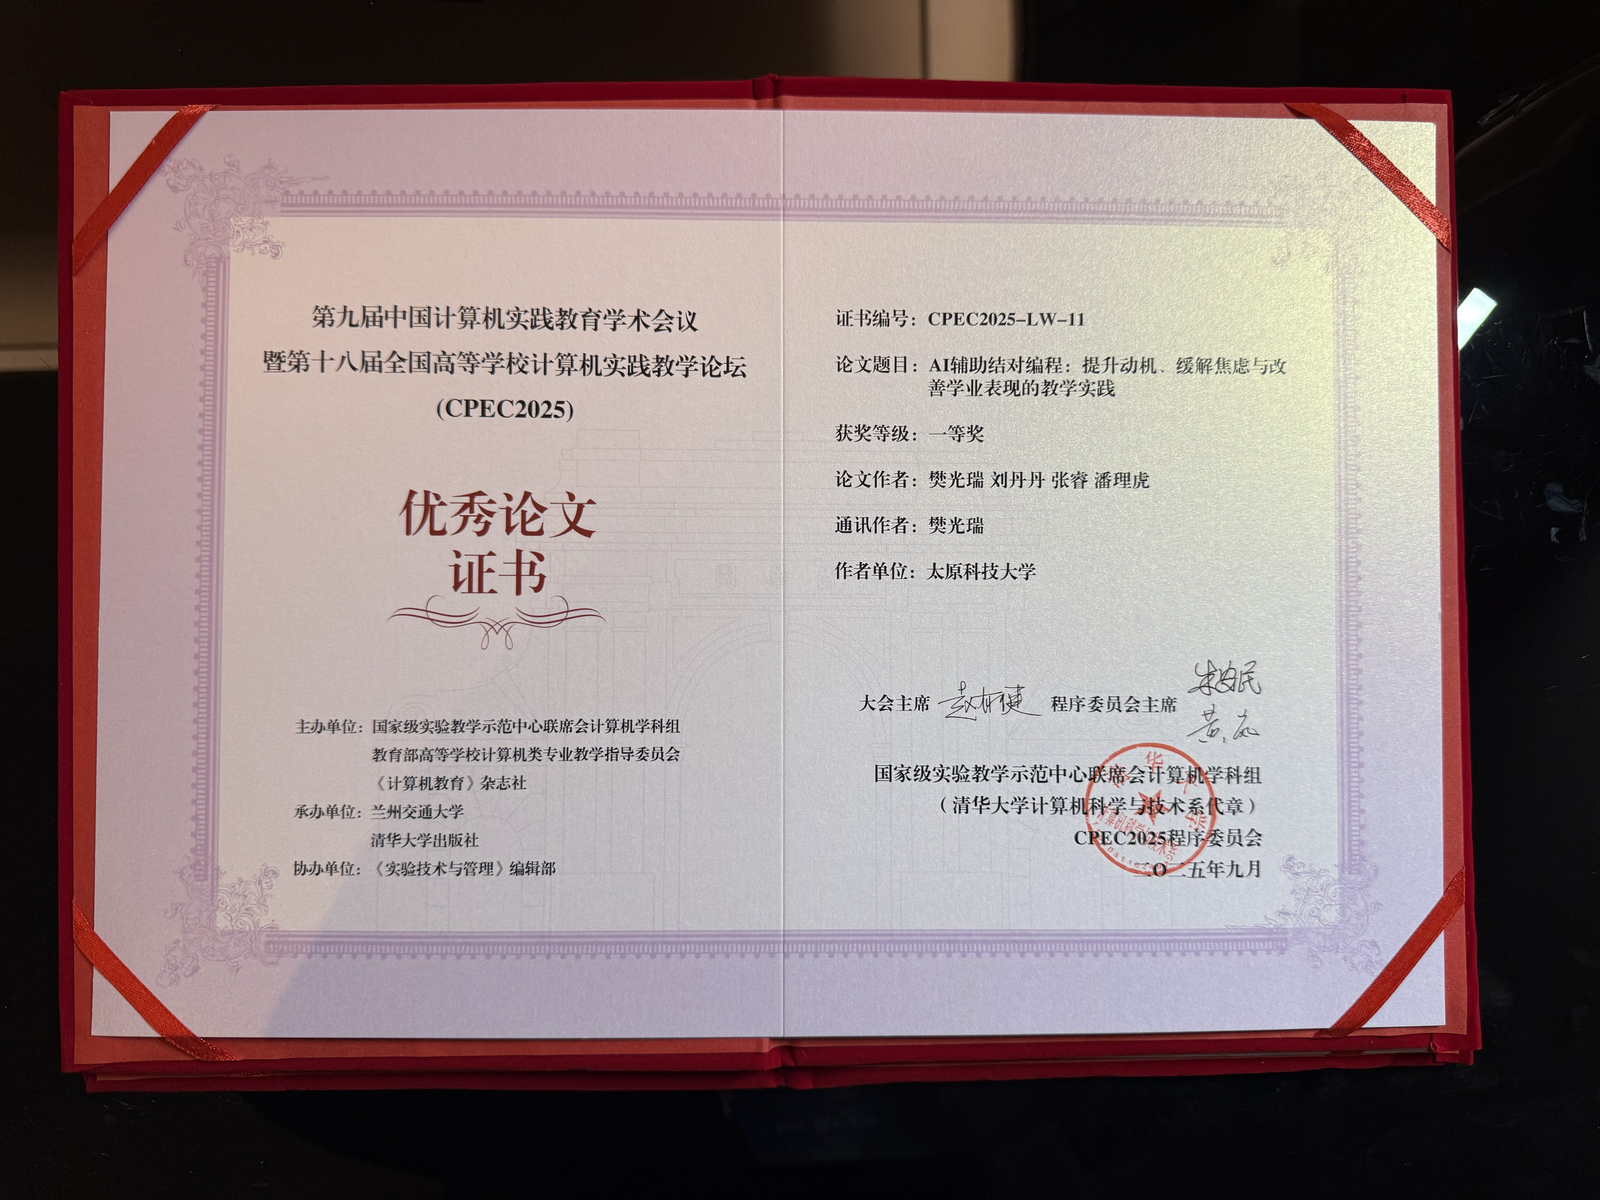
\includegraphics[width=\linewidth,height=4.05cm,keepaspectratio]{figures/award1_cpec_paper.png}\\
\scriptsize CPEC · Paper
\end{column}
\begin{column}{0.32\textwidth}
\centering
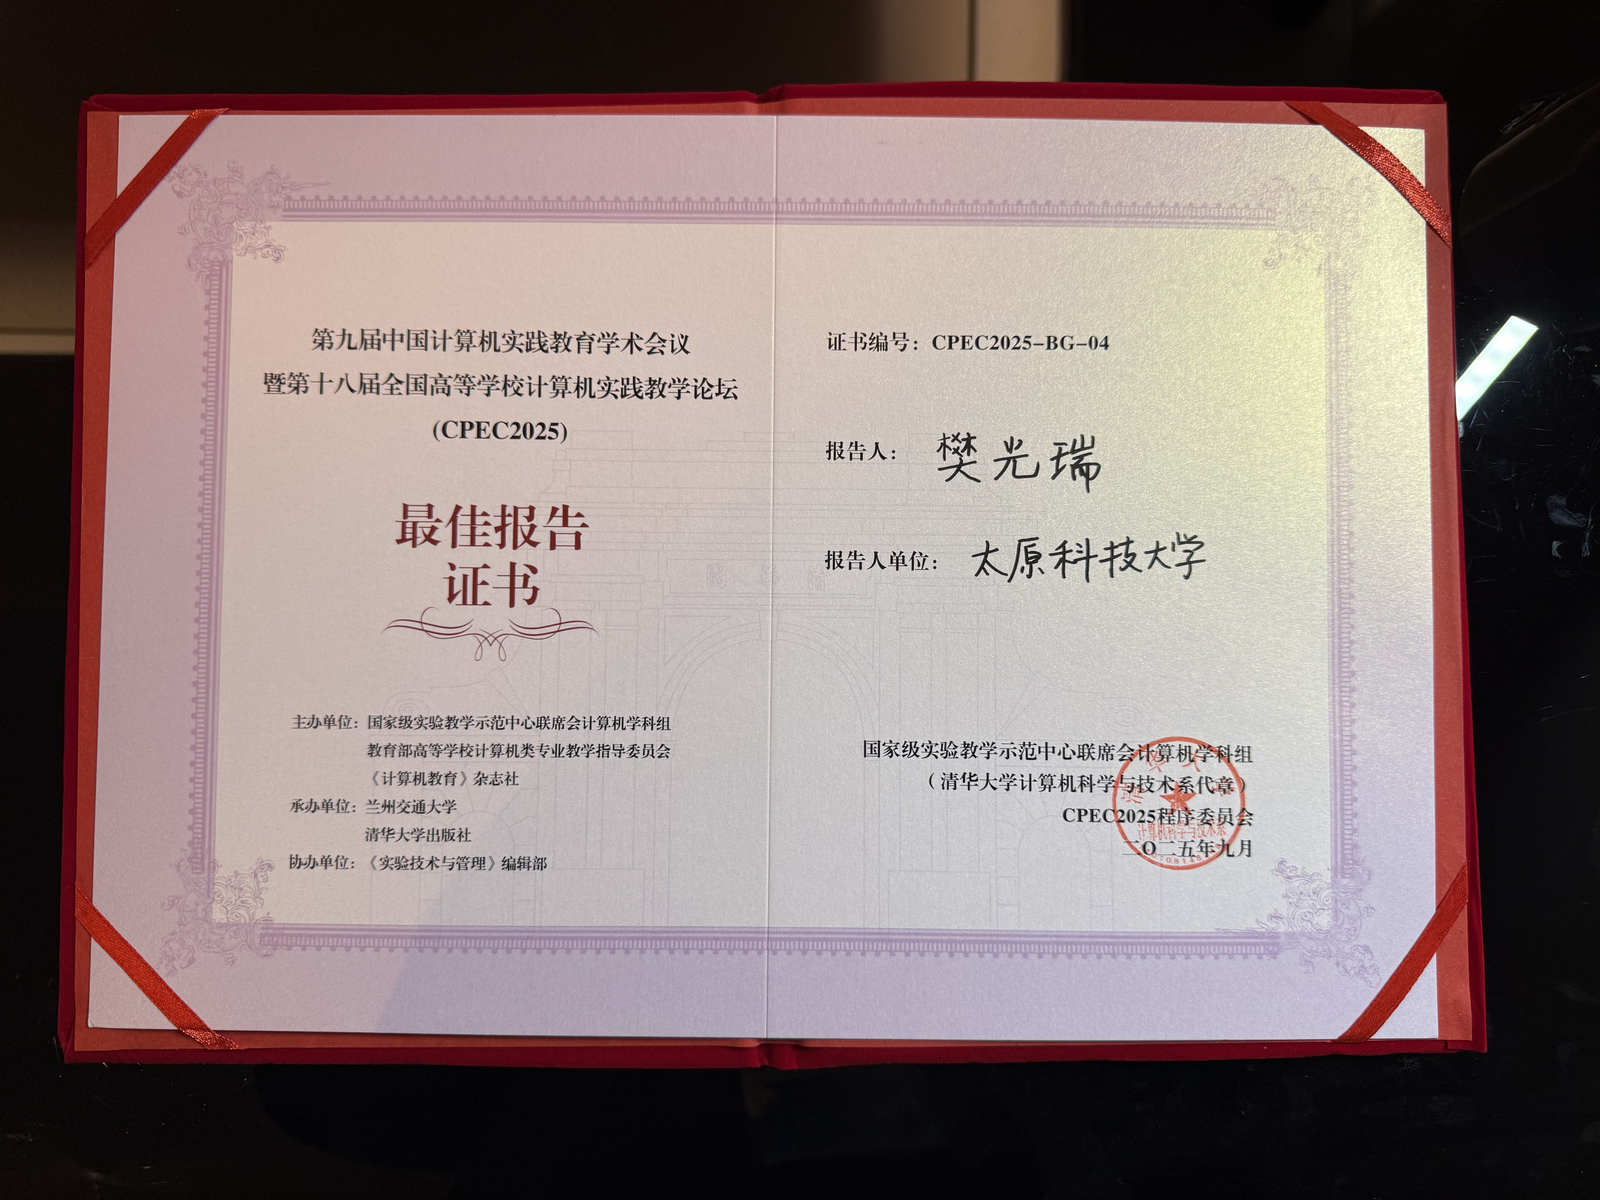
\includegraphics[width=\linewidth,height=4.05cm,keepaspectratio]{figures/award2_cpec_report.png}\\
\scriptsize CPEC · Report
\end{column}
\begin{column}{0.32\textwidth}
\centering
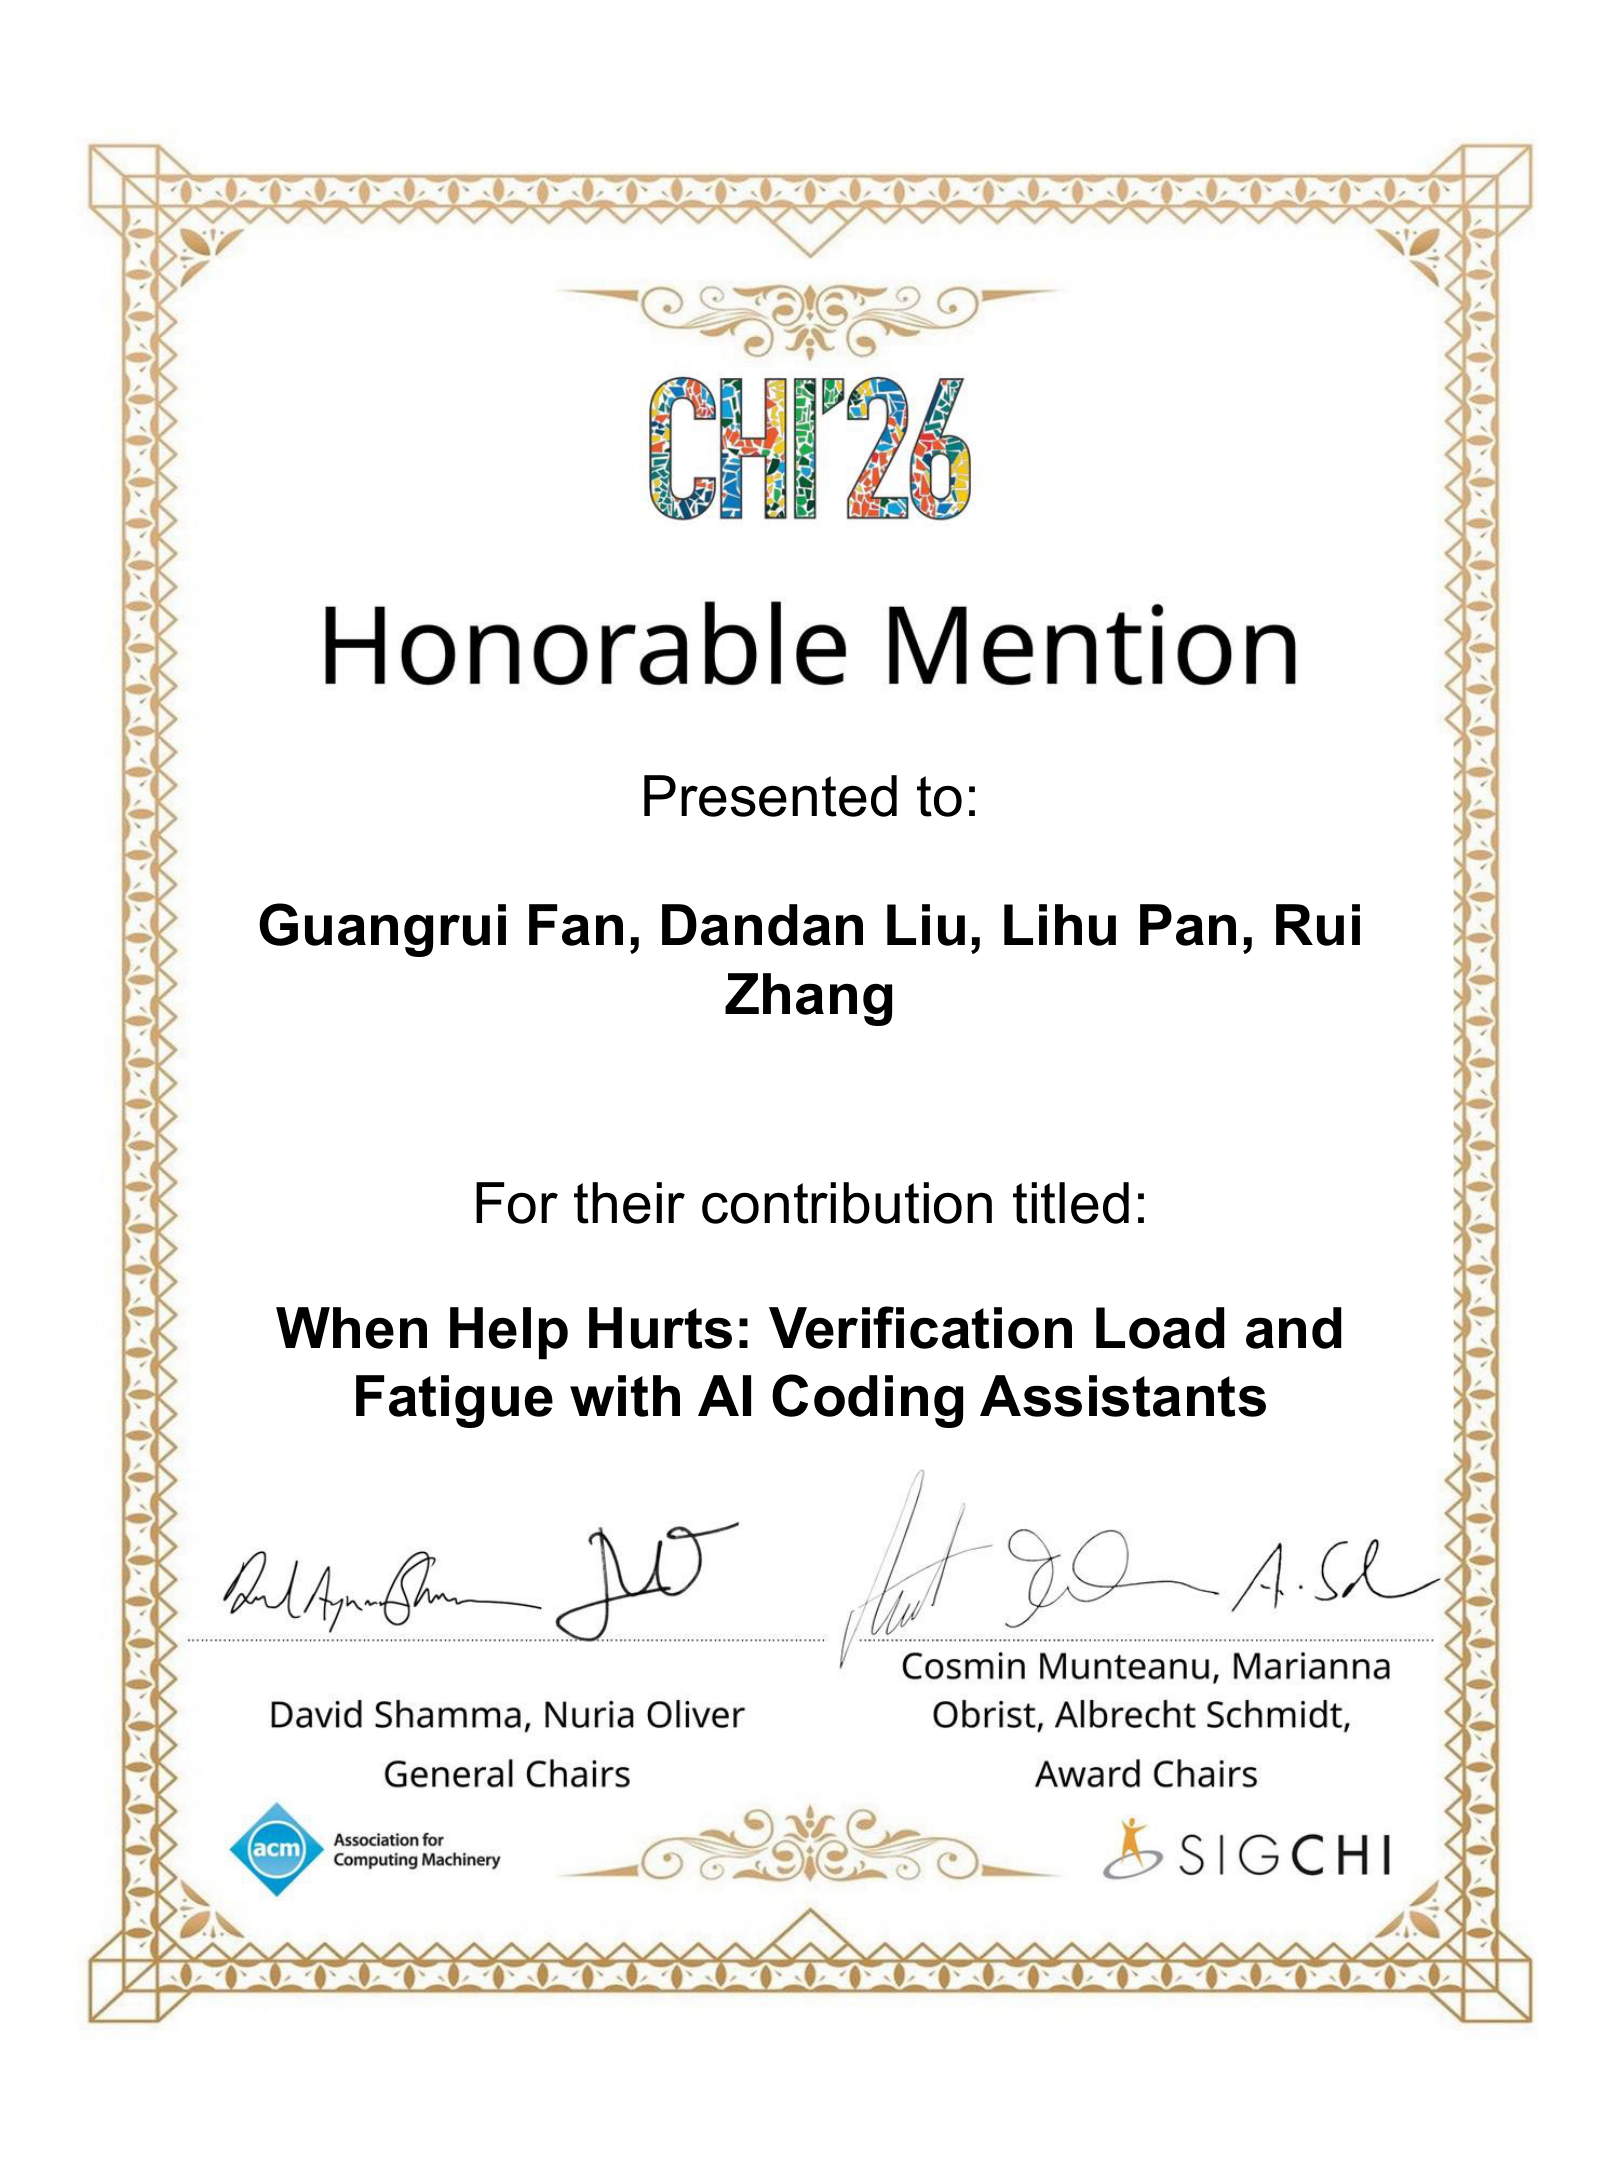
\includegraphics[width=\linewidth,height=4.05cm,keepaspectratio]{figures/award3_chi_hm.png}\\
\scriptsize CHI HM
\end{column}
\end{columns}
\end{frame}

% =====================================================================
\section{研究主线}

\begin{frame}{研究主线：HCI 驱动的人本可信 AI}
\begin{block}{Through-line}
研究 AI 系统进入真实场景后，如何改变人的 \hl{认知、协作、信任与选择}。
\end{block}
\vspace{2mm}
\begin{columns}[T]
\begin{column}{0.32\textwidth}
\textbf{人如何理解 AI}
\begin{itemize}\tightitems
  \item 作者身份
  \item 真实性
  \item 情感适宜性
  \item 隐私边界
\end{itemize}
\end{column}
\begin{column}{0.32\textwidth}
\textbf{人与 AI 如何协作}
\begin{itemize}\tightitems
  \item 编程助手
  \item 智能助教
  \item 虚拟焦点小组
  \item 人类反馈
\end{itemize}
\end{column}
\begin{column}{0.32\textwidth}
\textbf{AI 如何被评估}
\begin{itemize}\tightitems
  \item 用户实验
  \item 混合方法
  \item 可解释机器学习
  \item 公平与隐私审计
\end{itemize}
\end{column}
\end{columns}
\end{frame}

\begin{frame}{与目标学院方向契合}
\begin{itemize}\tightitems
  \item \textbf{HCI 与交互智能：}AI 进入真实场景后，用户如何理解、信任、协作与决策
  \item \textbf{AI 辅助软件工程与编程教育：}面向软件开发、需求分析、AI 编程助手与本科教学
  \item \textbf{可信 AI 与社会智能：}面向公平、隐私、心理健康、推荐与交通等高风险场景
\end{itemize}
\vspace{5mm}
\begin{block}{可合作方向}
把 HCI 用户证据、软件工程应用场景和 AI 方法创新放在同一条研究链上。
\end{block}
\end{frame}

% =====================================================================
\section{代表性研究}

\begin{frame}{方向一：HCI 与 AI 介导沟通}
AI 进入沟通与情感场景后，人如何重新判断 \hl{作者身份、情感规范与隐私边界}。
\vspace{3mm}
\small
\renewcommand{\arraystretch}{1.25}
\begin{tabularx}{0.96\textwidth}{@{}p{2.4cm}Yp{1.4cm}@{}}
\toprule
\textbf{Venue} & \textbf{Paper} & \textbf{Tier}\\
\midrule
CHI 2026 & \textbf{Is It Still You?} AI-Assisted Romantic Communication & CCF-A\\
ACL 2026 & \textbf{Feeling Rules in Language Models} & CCF-A\\
CHI 2026 & \textbf{Co-Adaptive Eco-Nudging} & CCF-A\\
ECSCW 2026 & \textbf{Consent Boundaries by Play} & CCF-B\\
\bottomrule
\end{tabularx}
\vspace{3mm}
\begin{block}{Finding}
透明披露与控制权回交可显著修复 AI 介入后的真实感与信任判断。
\end{block}
\end{frame}

\begin{frame}{方向一：代表性论文与图示}
\small
\begin{columns}[T]
\begin{column}{0.46\textwidth}
\figbox{figures/p1a_teaser.png}{0.43}\hfill
\figbox{figures/p1a_result.png}{0.43}
\vspace{2mm}

\paperbadge{CHI 2026 · CCF-A}\\
\textbf{Is It Still You?}\\
作者身份与真实性判断；三阶段判断模型；透明披露 + 控制权回交。
\end{column}
\begin{column}{0.46\textwidth}
\figbox{figures/p1b_teaser.png}{0.43}\hfill
\figbox{figures/p1b_result.png}{0.43}
\vspace{2mm}

\paperbadge{ACL 2026 · CCF-A}\\
\textbf{Feeling Rules in Language Models}\\
跨角色、机构、强度三维测度；高强度/机构权威情境下出现系统性偏移。
\end{column}
\end{columns}
\end{frame}

\begin{frame}{方向二：AI 辅助编程教育与认知负担}
AI 帮助 \hl{不等于} 自动减负；课程需要训练学生验证、解释与边界判断。
\vspace{3mm}
\small
\renewcommand{\arraystretch}{1.25}
\begin{tabularx}{0.96\textwidth}{@{}p{2.4cm}Yp{1.6cm}@{}}
\toprule
\textbf{Venue} & \textbf{Paper / Work} & \textbf{Remark}\\
\midrule
CHI 2026 & \textbf{When Help Hurts} & CCF-A · HM\\
IJ STEM Edu & \textbf{AI-Assisted Pair Programming} & Q1 Top · ESI\\
IJ STEM Edu & \textbf{Tool, Tutor, or Crutch?} & Q1 Top\\
Teaching & 课程内 AI 反馈系统、毕设指导与教学创新论文 & CPEC\\
\bottomrule
\end{tabularx}
\vspace{3mm}
\begin{block}{Concept}
提出 \hl{Verification Load}：失败、返工、上下文切换构成 AI 编程助手带来的新负担。
\end{block}
\end{frame}

\begin{frame}{方向二：代表性论文与图示}
\small
\begin{columns}[T]
\begin{column}{0.46\textwidth}
\figbox{figures/p2a_teaser.png}{0.43}\hfill
\figbox{figures/p2a_result.png}{0.43}
\vspace{2mm}

\paperbadge{CHI 2026 · CCF-A · HM}\\
\textbf{When Help Hurts}\\
Inline / Chat / Structured 三类交互模式对照；Structured 模式显著减压。
\end{column}
\begin{column}{0.46\textwidth}
\figbox{figures/p2b_teaser.png}{0.43}\hfill
\figbox{figures/p2b_result.png}{0.43}
\vspace{2mm}

\paperbadge{IJ STEM Education · Q1 Top · ESI}\\
\textbf{AI-Assisted Pair Programming}\\
本科生课堂对照实验；动机提升、焦虑下降、协作增强。
\end{column}
\end{columns}
\end{frame}

\begin{frame}{方向三：AI 辅助软件工程与人类反馈}
用 \hl{多 LLM 角色} 模拟真实用户，校正 \hl{网络采样的人类反馈} 偏差。
\vspace{3mm}
\small
\renewcommand{\arraystretch}{1.25}
\begin{tabularx}{0.96\textwidth}{@{}p{2.4cm}Yp{1.4cm}@{}}
\toprule
\textbf{Venue} & \textbf{Paper / Work} & \textbf{Tier}\\
\midrule
FSE 2026 & \textbf{Multi-LLM Persona Generation} for Virtual Focus Groups & CCF-A\\
ICML 2026 & \textbf{Graph-Preference Learning} & CCF-A\\
ICML 2026 & \textbf{Incomplete Multi-View Clustering} & CCF-A\\
Companion & 软件需求分析、人类偏好建模、多视图鲁棒学习 & Method\\
\bottomrule
\end{tabularx}
\vspace{3mm}
\begin{block}{Contribution}
从 HCI 用户研究出发，反向推动软件工程需求获取与机器学习偏好建模方法。
\end{block}
\end{frame}

\begin{frame}{方向三：代表性论文与图示}
\small
\begin{columns}[T]
\begin{column}{0.46\textwidth}
\figbox{figures/p3a_teaser.png}{0.43}\hfill
\figbox{figures/p3a_result.png}{0.43}
\vspace{2mm}

\paperbadge{FSE 2026 · CCF-A}\\
\textbf{Multi-LLM Persona Generation}\\
多 LLM persona + virtual focus groups；可控、可复现的用户模拟工具。
\end{column}
\begin{column}{0.46\textwidth}
\figbox{figures/p3b_teaser.png}{0.43}\hfill
\figbox{figures/p3b_result.png}{0.43}
\vspace{2mm}

\paperbadge{ICML 2026 · CCF-A}\\
\textbf{Graph-Preference Learning}\\
图上建模偏好结构 + 可学习重加权采样器；降低 welfare 估计误差。
\end{column}
\end{columns}
\end{frame}

\begin{frame}{方向四：可靠 AI、隐私与情感计算}
把公平、隐私、心理健康、情感等场景，变成 \hl{可解释、可评估、可治理} 的方法问题。
\vspace{3mm}
\small
\renewcommand{\arraystretch}{1.25}
\begin{tabularx}{0.96\textwidth}{@{}p{2.4cm}Yp{1.4cm}@{}}
\toprule
\textbf{Venue} & \textbf{Paper / Work} & \textbf{Tier}\\
\midrule
WWW 2026 & \textbf{Audit-of-Audits for the Web} & CCF-A\\
AAAI 2026 & \textbf{Mind the Gap} & CCF-A\\
IEEE TCSS & \textbf{Textless, Tiny, and Private} & CCF-C\\
EAAI & 可解释推荐、可信交通预测与隐私保护情感计算 & Q1\\
\bottomrule
\end{tabularx}
\vspace{3mm}
\begin{block}{Contribution}
用可解释模型与审计方法，让高风险 AI 场景中的信任问题变成可度量的研究对象。
\end{block}
\end{frame}

\begin{frame}{方向四：代表性论文与图示}
\small
\begin{columns}[T]
\begin{column}{0.46\textwidth}
\figbox{figures/p4a_teaser.png}{0.43}\hfill
\figbox{figures/p4a_result.png}{0.43}
\vspace{2mm}

\paperbadge{WWW 2026 · CCF-A}\\
\textbf{Audit-of-Audits for the Web}\\
分布式贝叶斯后验估计；主流平台公平性声明存在系统性高估。
\end{column}
\begin{column}{0.46\textwidth}
\figbox{figures/p4b_teaser.png}{0.43}\hfill
\figbox{figures/p4b_result.png}{0.43}
\vspace{2mm}

\paperbadge{AAAI 2026 · CCF-A}\\
\textbf{Mind the Gap}\\
解释在线心理健康社区 reply gap；关键支持时机可被预测和缩短。
\end{column}
\end{columns}
\end{frame}

% =====================================================================
\section{计划与总结}

\begin{frame}{成果总览}
\scriptsize
\renewcommand{\arraystretch}{1.12}
\begin{tabularx}{\textwidth}{@{}p{0.8cm}Yp{2.35cm}p{1.8cm}@{}}
\toprule
 & \textbf{方向} & \textbf{Venue} & \textbf{成果}\\
\midrule
01 & HCI 与 AI 介导沟通 & CHI · ACL · ECSCW & CCF-A ×3 + B\\
02 & AI 辅助编程教育与认知负担 & CHI · IJ STEM Edu & CCF-A + Q1 ×2\\
03 & AI 辅助软件工程与人类反馈 & FSE · ICML & CCF-A ×3\\
04 & 可靠 AI、隐私与社会智能 & WWW · AAAI · TCSS · EAAI & CCF-A ×2 + C + Q1\\
05 & 学术影响 & Honors & 1 CHI HM · 1 ESI 高被引\\
\bottomrule
\end{tabularx}
\vspace{2mm}
\smallmuted{\textbf{Summary:} 9 篇一作 / 通讯 CCF-A 顶会论文，4 篇中科院 1 区 Top SCI 期刊，研究与教学之间形成稳定互相支撑。}
\end{frame}

\begin{frame}{未来三年计划}
\small
\begin{columns}[T]
\begin{column}{0.32\textwidth}
\textbf{\textcolor{maincolor}{课程建设}}
\begin{itemize}\tightitems
  \item AI 编程助手实践课
  \item HCI 用户研究实验课
  \item 软件工程 × LLM 综合实践
\end{itemize}
\end{column}
\begin{column}{0.32\textwidth}
\textbf{\textcolor{maincolor}{科研方向}}
\begin{itemize}\tightitems
  \item 持续产出 CCF-A 论文
  \item 申报国家自然科学基金青年项目
  \item 与 SE / AI 团队联合攻关
\end{itemize}
\end{column}
\begin{column}{0.32\textwidth}
\textbf{\textcolor{maincolor}{学生培养}}
\begin{itemize}\tightitems
  \item 本科生进入 CHI / CSCW 投稿训练
  \item 研究生主导 HCI 用户研究
  \item 输送工业界与顶尖博士项目
\end{itemize}
\end{column}
\end{columns}
\vspace{4mm}
\begin{block}{目标}
把课程、科研与学生培养形成闭环，让课堂问题持续产生可发表、可应用、可指导学生成长的研究主题。
\end{block}
\end{frame}

\begin{frame}{谢谢各位老师}
\begin{center}
{\Large 期待围绕 HCI、AI 辅助软件工程与教学科研需求进一步交流。}

\vspace{10mm}
\textbf{樊光瑞 · Fan Guangrui}\\
PhD Candidate, Universiti Malaya\\
gerryfan2022@gmail.com\\
gerryfan0706.github.io
\end{center}
\end{frame}

\end{document}
